%Data Visualization Assignment 3: Project plan
%Author(s)		: Lukas Mirow
%Date of creation	: 2023-11-10

\documentclass[12pt, a4paper]{article}

\usepackage[utf8]{inputenc}
\usepackage[pdfauthor={Lukas Mirow}, pdftitle={Project Plan: An Analysis Of All 802 Pokemon Of The Generations 1 through 7}]{hyperref}
\usepackage{enumerate}
\usepackage{amsmath}
\usepackage{float}
\usepackage{graphicx}

\title{Project Plan: An Analysis Of All 802 Pokemon Of The Generations 1 through 7}
\author{Lukas Mirow}

\renewcommand{\labelitemi}{$\bullet$}
\renewcommand{\labelitemii}{$\bullet$}
\renewcommand{\labelitemiii}{$\bullet$}
\renewcommand{\labelitemiv}{$\bullet$}

\begin{document}
	\maketitle
	\tableofcontents
	\newpage

	\section{The Data Source}
		As described in the pitch of this project\footnote{Accessible on \href{https://ordpresse.0x.no/ass3-pres/}{https://ordpresse.0x.no/ass3-pres/} and on \href{https://lu6541196.azurewebsites.net/wp-content/uploads/2023/11/ass3-pres.pdf}{https://lu6541196.azurewebsites.net/wp-content/uploads/2023/11/ass3-pres.pdf}}, the data source will be \textit{The Complete Pokemon Dataset} available on \textit{Kaggle}.\footnote{Accessible on \href{https://www.kaggle.com/datasets/rounakbanik/pokemon}{https://www.kaggle.com/datasets/rounakbanik/pokemon}} The data source is available for download and is comprised of a CSV file, 150 KiB in size.

	\section{The Visualization Of The Data Set}
		\paragraph{}
			The data is to be visualized in two different ways: a table view and a comparison view. First, a characteristic can be chosen by the user on one of the tabs on the top of the table. Depending on the nature of the chosen characteristic, the remainder of the table will change.
		\paragraph{}
			\begin{figure}[h]
				\centering
				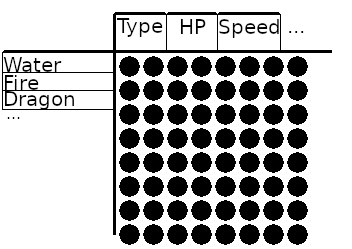
\includegraphics[width=0.5\linewidth]{table-ns.png}
				\caption{Table view for non-sortable characteristics}
				\label{fig:ns}
			\end{figure}
			If the chosen characteristic is not sortable; such as a category or a label, for example type or weakness; the table will show the possible categories or labels as check boxes on the left of the table and all Pokemon in a grid view, sorted by ID in the Pokedex in the body of the table. The Pokemon that are shown depend on which check boxes on the left of the table are checked. An example of this view for types is shown in figure \ref{fig:ns}.
		\pagebreak
		\paragraph{}
			\begin{figure}[h]
				\centering
				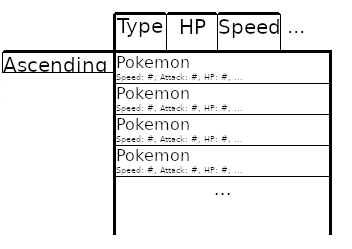
\includegraphics[width=0.5\linewidth]{table-s.png}
				\caption{Table view for sortable characteristics}
				\label{fig:s}
			\end{figure}
			If the chosen characteristic is sortable; such as numbers, for example speed or hit points; the table body will show a list of Pokemon, sorted by the chosen characteristic. Options as to how to sort these Pokemon can be changed at the top of the table. An example of this view for types is shown in figure \ref{fig:s}.
		\paragraph{}
			\begin{figure}[h]
				\centering
				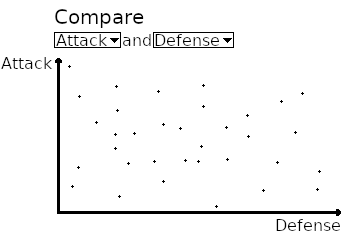
\includegraphics[width=0.5\linewidth]{comparison.png}
				\caption{Comparison of metric characteristics}
				\label{fig:c}
			\end{figure}
			The comparison view allows the user to choose two numerical characteristics from drop-down lists and shows all Pokemon on a scatter plot with these characteristics as axes. An example of this view for types is shown in figure \ref{fig:c}.
		\paragraph{}
			When the user clicks on any of these Pokemon representation, it opens a context window displaying all information given in the dataset.

	\section{The Target Audience}
		The target audience for this project includes individuals who have an interest in Pokemon and want to explore and analyze Pokemon characteristics in a visual and interactive manner. The target audience are people of all ages who have prior experience with the Pokemon franchise. This includes people that would like to satisfy their curiosity and people who play or played the video games and would like to use the data and comparing tools provided to gain insights or plan the composition of their Pokemon team. The project aims to be accessible as a website to desktop and mobile devices.

	\section{Synergy Of The Visualizations And The Story}
		The story that accommodates the visualizations revolves around how to tailor a Pokemon team toward a specific opponent's team given the types or specific Pokemon that this trainer uses. Since the Pokemon team that a non-player trainer in the Pokemon games has are pre-defined, it is possible to create a Pokemon team that is most effective in battling this trainer. A team tailored to beat the Elite Four and the Champion is created in the story accommodating the visualizations.

\end{document}
